\documentclass[a4paper, 11pt]{article}

\setcounter{tocdepth}{3}
\setcounter{secnumdepth}{3}

\usepackage{comment} % enables the use of multi-line comments (\ifx \fi) 
\usepackage{lipsum} %This package just generates Lorem Ipsum filler text. 
\usepackage{fullpage} % changes the margin
\usepackage[utf8]{inputenc}
\usepackage{gensymb}
\usepackage{graphicx}
\usepackage{booktabs}% http://ctan.org/pkg/booktabs
\usepackage{makecell}
\usepackage{tabularx}
\usepackage[table]{xcolor}
\usepackage{array}
\usepackage{wrapfig}
\usepackage{subcaption}
\usepackage{csquotes}
\usepackage{lscape}
\usepackage{afterpage}
\usepackage{geometry}
\usepackage{listingsutf8}
\usepackage{chngcntr}
\usepackage{multicol}
\usepackage{xcolor}
\usepackage{pifont}
\usepackage{makecell}
\usepackage{textcomp}


\counterwithin{figure}{section}

\geometry{a4paper, margin=1in}
\renewcommand{\figurename}{Abb.}
\renewcommand{\tablename}{Tabelle}
\newcommand{\code}[1]{\texttt{#1}}

\renewcommand*{\thead}[1]{\bfseries #1}

\renewcommand{\contentsname}{Inhalt}
\renewcommand{\listfigurename}{Abbildungsverzeichnis}

\definecolor{lightgray}{rgb}{.9,.9,.9}
\definecolor{darkgray}{rgb}{.4,.4,.4}
\definecolor{purple}{rgb}{0.65, 0.12, 0.82}
\definecolor{darkgreen}{rgb}{0.05,0.56,0.06}

\lstset{frame=tlrb,
    language=C,
    aboveskip=3mm,
    belowskip=3mm,
    showstringspaces=false,
    columns=flexible,
    basicstyle={\small\ttfamily},
    numbers=left,
    numberstyle=\tiny\color{gray},
    keywordstyle=\color{blue},
    commentstyle=\color{violet},
    stringstyle=\color{darkgreen},
    breaklines=true,
    breakatwhitespace=true,
    tabsize=3,
    literate=%
    {Ö}{{\"O}}1
    {Ä}{{\"A}}1
    {Ü}{{\"U}}1
    {ß}{{\ss}}1
    {ü}{{\"u}}1
    {ä}{{\"a}}1
    {ö}{{\"o}}1
}

\graphicspath{{img/}}


\begin{document}

\title{Zusammenfassung C}
\maketitle

\tableofcontents

\newpage

\section{Introduction}

C is a programming language, probably most known for being used to write and extend the UNIX Operating System.

It was originally developed by Dennis M. Ritchie in 1972 and remains one of the most used high level programming languages today (next to Java).

A 'C'-File should have the file-extension \code{.c} and must contain at least the following lines:

\begin{lstlisting}
#include <stdio.h>
int main(){
}
\end{lstlisting}

\section{Hello World}
\begin{minipage}{0.6\textwidth}
    The codeblock to the right shows a simple 'Hello World' program. All it does it print out 'Hello World' on the console, once compiled and run.
\end{minipage}\hfill
\begin{minipage}{0.35\textwidth}
    \begin{lstlisting}
#include <stdio.h>
int main(){
    printf("Hello World");
    return 0;
}
    \end{lstlisting}
\end{minipage}

The first line of this program \code{\#include <stdio.h>} tells the C-compiler to include the stdio header file before compiling the actual file.

The \code{int main()} is the main-method. The program execution starts there.

\code{return 0} terminates the main method and returns the value 0, usually interpreted as 'Everything worked fine'

\vspace{10px}

To run this file, you first have to compile it. Assuming you saved the file as \code{hello.c} and run Linux, you just have to open a console and run \code{gcc hello.c}. This command uses the GNU-C-compiler to compile your C-file. It will generate a file called \code{a.out} (you can change this by specifying a file name with the \code{-o}-Parameter, e.g. \code{gcc hello.c -o hello.compiled}).

\section{Identifiers}
An identifier is a name for a variable or a function. C allows basically all alphanumerical names, as long as they start with a letter or an underscore ('\_'). So \code{abc123} would be a legal variable name, as would be \code{\_11abc}. However \code{1\_ab\#d} would not be. 

\vspace{10px}


\textbf{Important:} C is case sensitive, so variable \code{variable} is not the same as \code{VaRiaBlE}.

\vspace{10px}

I'm saying 'basically', because C has reserved some words for language-specific things. These words are:

\begin{lstlisting}
auto 	else 	long 	switch      break 	enum 	register 	typedef     case 	extern 	return 	union   char 	float 	short 	unsigned    const 	for 	signed 	void   continue 	goto 	sizeof 	volatile    default 	if 	static 	while   do 	int 	struct 	_Packed    double
\end{lstlisting}

\newpage

\section{Data Types}
C uses different data types for different things. The type of a variable determines how much space it occupies in storage and how the bit pattern stored is interpreted.

C-Types can be classified as follows:

\begin{description}
    \item[Basic Types: ] Arithmetic Types ('You can do math with them'). Are further classified into \\
        \textit{a: Integer Types} \\
        \textit{b: Floating-point Types}
    \item[Enumerated Types: ] Arithmetic Types, used to define variables that can only assign certain integer values. (i.e enums)
    \item[Void Types: ] No value
    \item[Derived Types: ] Further divided into \\
        \textit{a: Pointer Types} \\
        \textit{b: Array Types} \\
        \textit{c: Structure Types} \\
        \textit{d: Union Types} \\
        \textit{e: Function Types}
\end{description}

\subsection{Integer Types}

\begin{table}[htpb]
    \centering
    \caption{Integer Types, their storage size and value range}
    \label{tab:int-storage}
    \begin{tabular}{|c|c|r|}
        \hline
        \thead{Type} & \thead{Storage Size}  & \thead{Value range} \\
        \hline
        char & 1 byte & -128 - 127 / 0 - 255 \\
        \hline
        unsigned char & 1 byte & 0 - 255 \\
        \hline
        signed char & 1 byte & -128 - 127 \\
        \hline
        int & 2-4 bytes & \makecell{-32'768 - 32'767 \\ -2'147'483'648 to 2'147'483'647} \\
        \hline
        unsigned int & 2-4 bytes & \makecell{0 - 65'535 \\ 0 - 4'294'967'295} \\
        \hline
        unsigned short & 2 bytes  & 0-65'5535 \\
        \hline
        short & 2 bytes & -32768 - 32767 \\
        \hline
        long & 8 bytes & -9'223'372'036'854'775'808 -  9'223'372'036'854'775'807 \\
        \hline
        unsigned long & 8 bytes & 0 - 18'446'744'073'709'551'615 \\
        \hline
    \end{tabular}
\end{table}

Alternatively, you can use the \code{sizeof} to get the size of a type (e.g. \code{sizeof(int)}) or just the stored values in the header-files (e.g. \code{LONG\_MAX})

\subsection{Floating-point Types}

\begin{table}[htpb]
    \centering
    \caption{Integer Types, their storage size and value range}
    \label{tab:int-storage}
    \begin{tabular}{|c|c|r|r|}
        \hline
        \thead{Type} & \thead{Storage Size}  & \thead{Value range} & \thead{Precision} \\
        \hline
        float & 4 byte & 1.2E-38 - 3.4E+38 & 6 decimal places \\
        \hline
        double & 8 byte & 2.3E-308 - 1.7E+308 & 15 decimal places \\
        \hline
        long double & 10 byte & 3.4E-4932 to 1.1E+4932 & 19 decimal places \\
        \hline
    \end{tabular}
\end{table}

\subsection{Void Types}

\begin{description}
    \item[Function returns as void: ] The function does not return anything.
    \item[Function arguments as void: ] The function does not take any parameters.
    \item[Pointers to void:] A pointer can point to a memory-address, but it does not have a type associated to it. You can store at that address whatever you want, given there's enough space for it.
\end{description}

\section{Variables}

\begin{minipage}{0.50\textwidth}
    Variables are basically just a name given to a memory-address, so it can be accessed more easily. Each variable has to be assigned to a specified type (char, int, float, double or void). 

    Variables can be defined, as in most other programming languages, with the '=' operator. (\code{int i = 3}). Multiple variables can be separated with a comma (\code{int i, j, k}). 

    If a C-program consists of multiple files, the compiler can be assured of the existence of a given variable with the \code{extern} keyword. It might not have been initialized yet, but it will, so an address-space must be allocated. 

    \subsection{Lvalues and Rvalues}

    \begin{description}
        \item[lvalue: ] Refers to a memory-address. Can be used on both sides of an assignment (\code{a=b})
        \item[rvalue: ] Refers to the data value at a memory-address. Can only be used on the right-hand side of an assignment (\code{a=20})
    \end{description}
\end{minipage}\hfill
\begin{minipage}{0.45\textwidth}
    \begin{lstlisting}
    #include <stdio.h>

    // Variable declaration:
    extern int a, b;
    extern int c;
    extern float f;

    int main () {

       /* variable definition: */
       int a, b;
       int c;
       float f;

       /* actual initialization */
       a = 10;
       b = 20;

       c = a + b;
       printf("value of c : %d \n", c);

       f = 70.0/3.0;
       printf("value of f : %f \n", f);

       return 0;
    }
    \end{lstlisting}
\end{minipage}

\subsection{Constants and Literals}

Constants, also called Literals are read-only variables. They are defined once and cannot be changed by the program. This can e.g. be useful for physical constants. The gravity will most likely not change during the runtime of the program. Constants usually refer to the rvalue of the actual value of the constant (rvalue), whereas literals are usually the address of said value (lvalue).

Constants can be defined as hexadecimal (prefix \code{0x}), octal (prefix \code{0}) or decimal (no prefix) values. They can also be unsigned (suffix \code{U}) or long (suffix \code{L}). 




\vspace{10px}
\begin{minipage}{0.45\textwidth}
    Constants can also be Float (\code{3.14159}, \code{314159E-5L}) or even chars. C already defines some char literals, which are preceded by \code{\textbackslash} (e.g. \code{\textbackslash t} or \code{\textbackslash n}).

    Constants can either be defined with the \code{\#define} preprocessor, or alternatively with the \code{const} keyword. 
\end{minipage}\hfill
\begin{minipage}{0.45\textwidth}
    \begin{lstlisting}
    #define PI 3.14159

    int main(){
        const float G = 9.81;
        printf("Gravity: %f \n", G);
        printf("Pi: %f", PI);
    }
    \end{lstlisting}
\end{minipage}

\section{Storage Classes}

Storage classes define the visibility, scope and lifetime of a variable or function.

\begin{description}
    \item[auto: ] Default - Only visible within the function (i.e. local variables)
    \item[register: ] Local variables which are to be stored in a register instead of memory. It can be accessed faster, but its size is limited to the register size (usually one word).
    \item[static: ] Global variable - Is kept alive throughout the whole program-execution. Alternatively, it can also mean that it is not destroyed and re-initiated after every function call.
    \item[extern: ] Variable visible to \textbf{all} program files.
\end{description}

\section{Operators}

The following tables/images show the different operators supported by C. 



\begin{figure}[htb!]
    \centering
    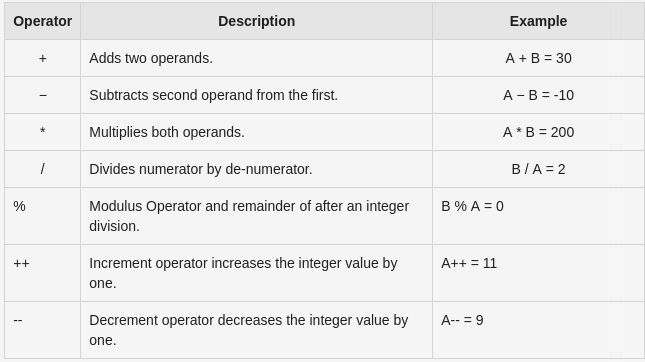
\includegraphics[width=0.8\textwidth]{arith_oper}
    \caption{Arithmetic Operators (Assume A holds 10 and B holds 20)}
    \label{fig:arith_oper}
\end{figure}

\newpage

\begin{figure}[htb!]
    \centering
    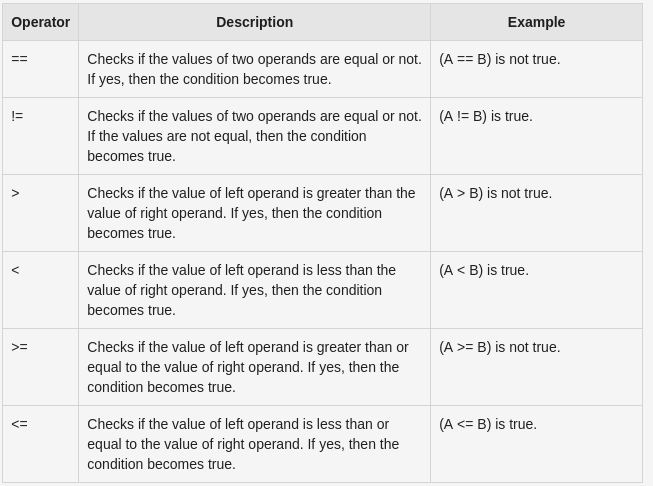
\includegraphics[width=0.8\textwidth]{relat_oper}
    \caption{Relational Operators (Assume A holds 10 and B holds 20)}
    \label{fig:relat_oper}
\end{figure}

\begin{figure}[htb!]
    \centering
    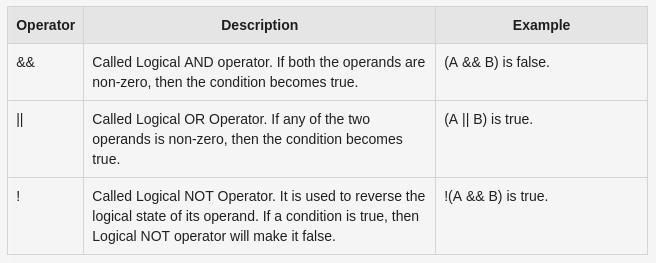
\includegraphics[width=0.8\textwidth]{log_oper}
    \caption{Logical Operators (Assume A holds 1 and B 0)}
    \label{fig:log_oper}
\end{figure}

\begin{figure}[htb!]
    \centering
    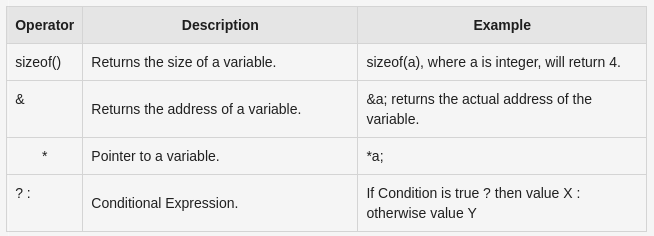
\includegraphics[width=0.8\textwidth]{misc_oper}
    \caption{Miscellaneous Operators}
    \label{fig:misc_oper}
\end{figure}

\newpage

\begin{figure}[htb!]
    \centering
    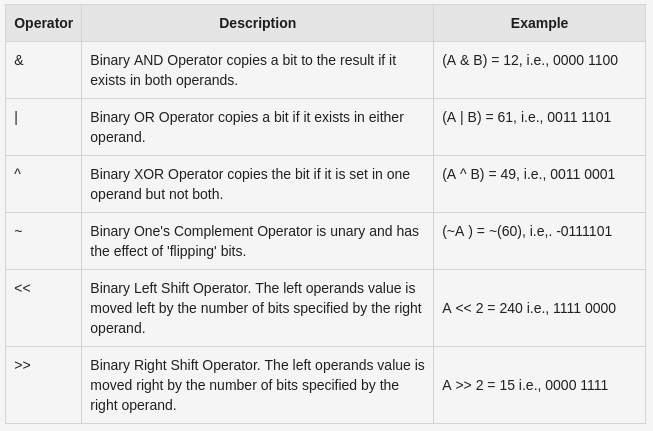
\includegraphics[width=0.8\textwidth]{bit_oper}
    \caption{Bitwise Operators (Assume A holds 60 and B 13)}
    \label{fig:bit_oper}
\end{figure}

\begin{figure}[htb!]
    \centering
    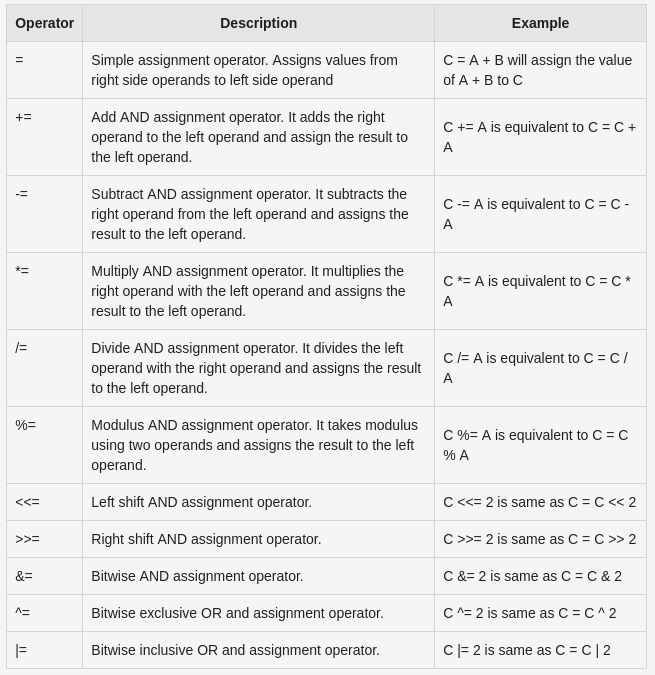
\includegraphics[width=0.8\textwidth]{assign_oper}
    \caption{Assignment Operators}
    \label{fig:assign_oper}
\end{figure}

\newpage

\begin{figure}[htb!]
    \centering
    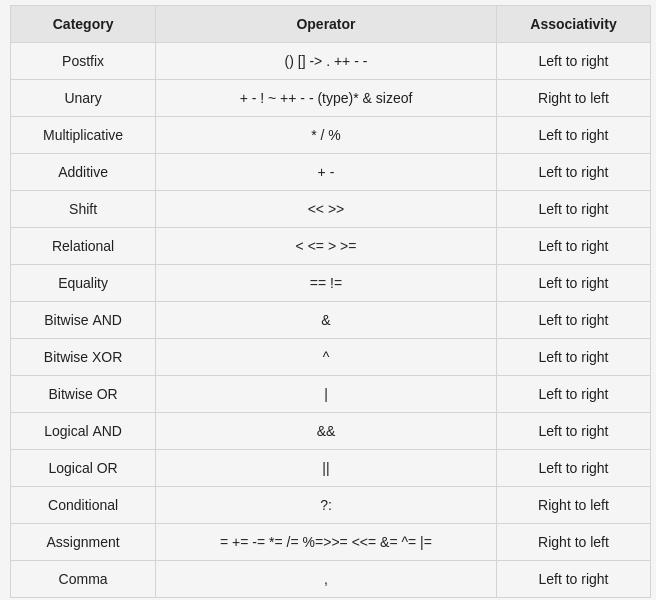
\includegraphics[width=0.8\textwidth]{oper_precedence}
    \caption{Operator Precedence (Top to Bottom as importance)}
    \label{fig:oper_precedence}
\end{figure}

\newpage

\section{Decision-Making}

As most other programming languages, C can choose one or another path depending on how or if a condition is met:

\begin{description}
    \item[if: ] Boolean expression followed by one or more statements, which are only executed if the boolean expression is true \\
        \begin{lstlisting}[frame=none, numbers=none]
           if(PI ==  3.14159 ){
                printf("Pi is set correctly");
           }
        \end{lstlisting}
    \item[if\ldots else: ] An if statement can have an optional 'else' block, which will only be executed if the boolean expression is false. \\
        \begin{lstlisting}[frame=none, numbers=none]
        if(PI ==  3.14159 ){
            printf("Pi is set correctly");
        } else {
    #define PI 3.14159
            printf("Pi has been set to the correct value");
        }
        \end{lstlisting}
    \item[nested ifs: ] If\ldots else statements can also be nested, so that if one statement holds true, the next one gets checked etc.
    \item[switch: ] A variable is being tested against a list of predefined values. \\
        \begin{lstlisting}[frame=none, numbers=none]
        switch(grade) {
        case 'A':
            printf("Excellent! \n");
            break;
        case 'B':
            printf("Good!");
            break;
        default:
            printf("Invalid grade");
        }
        \end{lstlisting}
    \item[nestd switch: ] Same as if-statements, switch statements can be nested as well.
    \item[?:-Operator: ] Shorthand for if\ldots else. \code{Exp1} is checked. If it is true, \code{Exp2} is checked and becomes the value of the entire expression. If \code{Exp1} is false, \code{Exp3} is checked and becomes the value of the entire expression \\
        \begin{lstlisting}[frame=none, numbers=none]
            /* if-else */
            if(a > b){
                result = x;
            } else {
                result = y;
            }

            /* same thing with ?: */
            result = a > b ? x : y;
            \end{lstlisting}

\end{description}

\end{document}
